\chapter{Informing implementation discussions}\label{chap:inform-impl}

In the early stages, \kl{CN} was implemented by Christopher Pulte and Thomas
Sewell, based on sketches by Neel Krishnaswami. I started formalising
\kl{Kernel CN} much later, and benefited by the clarity of having an
implementation and implementers I could consult in moments of
confusion.

However, this mode of development means that there were \emph{many} design
decisions made in a rather conservative context, because the programming was
always of a system which was being defined along the way, rather than a
well-understood pre-existing one. Extensions to syntax and inference were
always the minimum required for verifying the pKVM buddy allocator, lest
performance and inference suffer greatly, rather than ones based on a strong
formal and holistic consideration of the constructs and interactions at play.

As such, there are several restrictions in the implementation, which with the
benefit of hindsight and formalisation, are completely unnecessary, but persist
as technical debt. This chapter lists a few of these, and explains how the
formalisation brings much needed clarity to many questions around the
implementation.

\url{https://github.com/rems-project/cerberus/labels/language}
\url{https://github.com/rems-project/cerberus/labels/resource\%20reasoning}

\section{Supporting partially initialised reads of structs/unions}\label{sec:partial-init-structs}

So far in working on verifying the buddy allocator, writing a tutorial and
working with our industry partners, no code has needed the ability to read a
partially (including completely) uninitialised struct/union, and any valid code
which does this would have to simply ignore that result. The \kl{UB} only comes
when one tries to read an uninitialised primitive type member of the
struct/union from that earlier read.

Because we can decompose ownership of a struct into its fields, and track the
initialised status of those individually (perhaps verbosely for large structs),
it does not seems like we lose much in expressiveness in forbidding this. The
only valid code that would be additionally rejected if this was forbidden in
the type system would be a read of a partially initialised struct followed by a
call to a function which reads only the initialised fields. And in such
instances, it seems likely that the code could be refactored to only pass the
initialised fields, or a pointer with the appropriate precondition to only read
the initialised fields.

Although we wish to verify C code as is, because programmers need to change the
``code'' to write annotations anyway, such small, rare and easy to explain
refactors are a worthwhile trade-off if it makes the design and implementation
of \kl{CN} simpler. The book-keeping for tracking initialised status in
symbolic terms, rather than in a flag the name of a predicate, adds a
non-trivial amount of noise to formalisation and would do the same in the
implementation.

Perhaps such an allowance simplifies data-flow analysis inside a compiler, so
that it may safely ignore the values resulting from a load of partially
uninitialised loads of a of struct, so long as none of the fields are accessed.
It seems hard to think of a case for this allowance motivated by performance or
programmer ergonomics, and so the experience from formalising this suggests
that the current implementation of \kl{CN}, which does not allow loads from
partially (including completely) uninitialised structs, can and will remain
expressive enough for all of its use cases.

\section{Auto unfolding scheme for logical functions}\label{sec:auto-unfold-functions}

\url{https://github.com/rems-project/cerberus/issues/483}

One of the strange parts of working with \kl{CN} is the predicate definitions are
automatically unfolded but not logical functions, even though both may be
recursive. As such there is separate and cumbersome annotation to manually
unfold a function.

The way the implementation determines whether to unfold a predicate is
to always unfold it if there is no top-level if, or to check if the condition
or its negation can be proven before unfolding the corresponding branch.

However, with the benefit of the formalisation, we can see that those are
actually two orthogonal questions, which happen to be tied together because of
historical reasons. In the formalisation (\cref{fig:typing-res-pat}), including
the elaboration rules (\cref{fig:kernel-elab-fold}),  we can see that (un)folding % chktex 36
predicates does not require calling the SMT solver, but determining which
branch of an ordered-disjunction to check does.

So not only does this suggest loosening the restrictions on branching in
predicate definitions (\cref{sec:restriction-branching}), it also suggests that
the general approach of ``unfold until you reach a condition for which neither
it nor its negation can be proven'' would work for logical functions too.

It is important to note that with automatic constraint-based unfolding, it is
possible for users to write constraints (including via control flow) which make
\kl{CN} diverge, and at this stage it is unclear how any well-foundedness
checks on the definitions of predicates would prevent this particular failure
mode.\sidenote{\url{https://github.com/rems-project/cerberus/issues/451}}

\section{Higher-order resources}
\url{https://github.com/rems-project/cerberus/issues/363}

If we want \kl{CN} to be used in real-world settings, it must support
concurrency. We can use the formalisation to reflect on what changes
would be needed to support this.

Fractional permissions would be useful to enable sharing. After that,
the issue becomes what level of support would be useful and worth implementing
based on the size of the change.

For example, hard-coding support for locks as an extra kind of resource would
be relatively straightforward (adding more terms and operations to the
grammar), but adding support for higher-order resources in general, so that
locks can be defined rather than an built-in feature, would be substantial
change to the resource type definitions and rules.

\section{Restrictions on branching}\label{sec:restriction-branching}
\url{https://github.com/rems-project/cerberus/issues/483}
\url{https://github.com/rems-project/cerberus/issues/266}

As mentioned in~\nameref{sec:auto-unfold-functions}, the formalisation
separates out two features (unfolding definitions, and selecting a branch of an
ordered-disjunction) which are tied together in the implementation. One of
the other places this shows up is in a restricted syntax for predicate definitions:
they must either have no ordered-disjunctions, or only one, placed first at the
top-level.

With the formalisation, not only can I show that that restriction is
unnecessary, I can also shed light on how to change the implementation to lift it.

This is because I can argue that the surface syntactic restriction and the
internal representation of predicate definition are actually two
\emph{orthogonal} issues. The key insight here is that this feature does not
add any extra expressive power, it simply unbundles to features which are
orthogonal in the formalisation. Indeed, users can work around the restriction
by manually defining an extra auxiliary predicate each time they wish to use an
ordered-disjunction anywhere which is not first and at the top-level, it is just
clunky.

This orthogonality extends to implementing fixes for this issue too
\textemdash{} I can sketch out two ways of lifting this restriction in the
implementation and offer those options, with their own trade-offs, to other
developers and users to decide which, if any, is preferable.

\section{Removing the pointer first restriction on predicates}\label{sec:rm-ptr-first}
\url{https://github.com/rems-project/cerberus/issues/303}

Another awkward restriction in working with \kl{CN} is that the first argument
to a predicate must always be a pointer. This is usually fine because it would
be strange to speak of ownership without a pointer, but the pointer is derived
from elsewhere (a fixed base pointer, but a given index), or sometimes the
pointer is in a record and that is the easiest thing to pass in.

With the formalisation, we can estimate the impact of removing this restriction
and see that the main thing we would lose is not in terms of typing fewer
programs, but in terms of synthesising indices for manipulating iterated
predicates (\cref{subsec:synth-indices}). Given that \kl{CN} has already moved
away from inferring those,\sidenote{See note~\ref{sn:new-inf-statics}.} we can
conclude that removing this restriction will not diminish the automation or the
expressive power of \kl{CN}.\sidenote{It will not increase expressiveness
either, because users currently can and do just use a dummy parameter.}

\section{Unifying the syntax of functions, predicates and specifications}

\url{https://github.com/rems-project/cerberus/issues/304}

Syntax is part of the user-interface of \kl{CN}, and as such it is subject to
strong constraints, strong scrutiny and strong opinions.

Currently, logical (ghost) functions and predicates are separated (represented
by different OCaml types) in the implementation. This is with good reason:
the pure parts are shipped off to an SMT solver, but the heap parts are the
domain of the resource reasoning. However, \kl{CN} also enforces this
distinction syntactically, which is a perfectly valid choice, but it trades
concision and occasional confusion when those worlds need to mix, for clarity
in separating when the two do not.\sidenote{\url{https://github.com/rems-project/cerberus/issues/288}}

Another equally valid choice would be to unify the two syntaxes and find some
other way of enforcing the necessary distinction between the two worlds.
Exposing the monad implicit in the predicate syntax as a type constructor would
achieve both, though at the cost of exposing developers to a fancier type
system. As a programming-language theorist, I prefer this, though the ultimate
arbiter of such a decision would have to well-designed user-studies.

\chapter{An alternative presentation}\label{chap:kernel-alternative}

I will conclude this part by sketching out an alternative presentation of the
\kl{CN} type system, \intro{MiniCN}, closer to both C as a surface language and
the \kl{CN} implementation. It will demonstrate the challenges of \emph{not}
using \kl{ResCore}, due to it not being a first-order functional
language with explicit resources and let-normalisation. The former means the
inference cannot be specified separately, whereas the latter in particular
complicates typing early-returns and join-points. It will also demonstrate the
challenges which seem to be inherent to designing a type system for a C-like
language.

\section{MiniC and MiniCN}

\kl{MiniC} is a C-like language intended to capture the parts of C relevant to
explaining the core ideas behind
\intro{Fulminate}\sidecite{banerjee2025fulminate}, a separation-logic testing
framework which translates \kl{CN} specifications to C. It includes global
variables, mutable function paramaters, block-scoped local variables, and early
return, but omits loops and unstructured control flow such as \cinline{goto}.
Expressions and statements are unified into a single construct, and evaluation
is fixed to be left-to-right. The only MiniC types are integers or pointers
(with free conversion between the two), hence no structured data such as
structs or arrays. Notably, \kl{MiniC} includes taking the address of
variables, indirect assignment and dereferencing arbitrary expressions. Its
expression grammar is shown in \cref{fig:minic-grammar}.

\begin{figure*}[tp]
    \small
    \cngrammarcompressed{%
        \cndeclaration{}\cninterrule{}\\
        \cnblock{}\cninterrule{}\\
        \cnlvalueXXexpression{}\cninterrule{}\\
        \cnexpression{}\cninterrule{}\\
        \cnfuncXXdef{}\cnafterlastrule{}\\
    }%
    \caption{Grammar for a C-like language, \kl{MiniC}.}\label{fig:minic-grammar}
\end{figure*}

I will omit discussion of the operational semantics of \kl{MiniC}, which is
explained in the Fulminate paper.

The specification language for \kl{MiniC}, is a simplified version of the
surface syntax of \kl{CN} (\cref{fig:surface-cn-syntax}). The simplifications
are to (a) equate pointers and integers (b) assume that all
{\small$\cnkw{Owned}$}s are always initialised and (c) ignore any other C types,
including structs and arrays (d) ignore iterated predicates.

\section{Aliasing requires linear resources}

Because syntactically different expressions may alias the same heap locations,
the type system still needs symbolic expressions and linear resources to track
permissions on reading and writing locations (there is no allocation and
destruction). This is visible in the spine judgement (\cref{fig:minicn-spine}),
which is used to \emph{check} the typing contexts against a specification:
postconditions for return expressions, preconditions for function calls.

\begin{figure*}[tpb]
    \ContinuedFloat*
    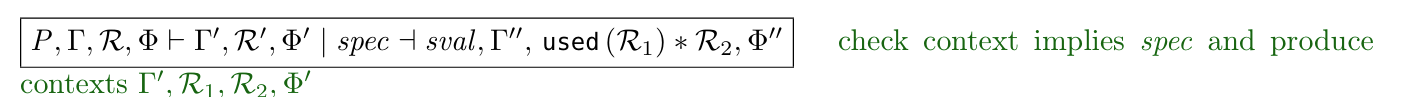
\includegraphics{figures/minicn-spine-1}
    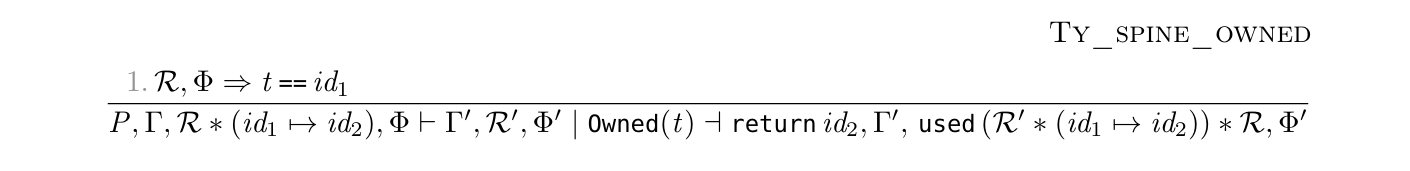
\includegraphics{figures/minicn-spine-2}
    \caption{Select spine judgement rules for \kl{MiniCN}.}\label{fig:minicn-spine}
\end{figure*}

The typing context includes: a program (list of definitions) $P$ for lookups,
$\Gamma$ for variables (computational and logical), a resource context
$\mathcal{R}$, and a constraint context $\Phi$. It accumulates contexts whilst
checking specification $\mathit{spec}$, and produces a specification value
$\mathit{sval}$, and contexts marking the new variables introduced, the
resources used and leftover, and additional constraints learned. I chose this
more complex accumulating style to mirror the (big-step) dynamic specification
checks.

The rule for checking ownership marks the resource in the context as
used\sidenote{I marked the resources as used and delete them at the use site,
instead of deleting them along the way, to mirror the dynamic semantics here
too.} if the location is proven to be equal.

\section{Implicit resources and terms intertwine elaboration and typing}

\kl{MiniCN} is intended to be closer to the syntax (and implementation)
than \kl{Kernel CN}. This is why I phrased the rules in terms of input and
output contexts, rather than the substructural kind. It also means that there
are no explicit resource terms or logical (ghost) quantifier instantiations in
the syntax tree.

As such, the rules for checking (and assuming) a specification both have to
compute the instantiation of logical (ghost) quantifiers on-the-fly, whereas
this is separated into typing and elaboration in the \kl{Kernel CN}
presentation. This is why, in addition to outputting a modified resource
context, the spine judgement also outputs a specification value
$\mathit{sval}$, as well as the additional constraints learnt (and additional
variables used). This is best demonstrated in \cref{fig:minicn-spine-take},
where (a) the bound expression $\mathit{t}$ is the result of
checking/evaluating $\mathit{spec}$ (b) the bound variable $\mathit{id}$ is
added to the accumulating variable context (c) their equality is added to the
accumulating constraint context before (d) checking/evaluating the rest of the
specification.

\begin{figure*}[tpb]
    \ContinuedFloat{}
    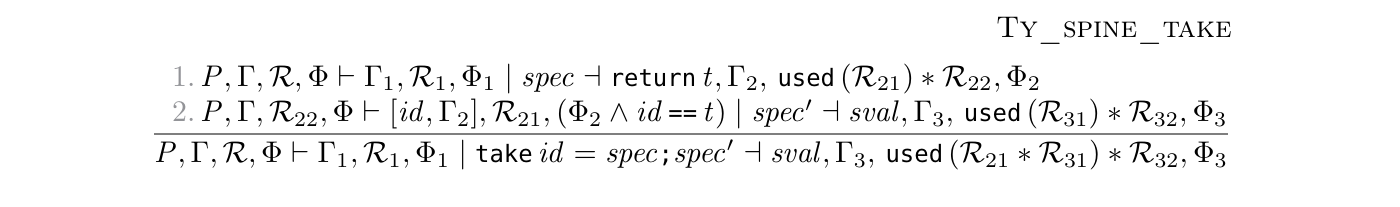
\includegraphics{figures/minicn-spine-3}
    \caption{Select spine judgement rules for \kl{MiniCN}.}\label{fig:minicn-spine-take}
\end{figure*}

\section{Early returns intertwine normalising, synthesising and checking}

Because expressions and statements are a single construct in \kl{MiniC}, and
statements include \cinline{return} statements, any expression could
potentially have its evaluation interrupted a nested early-return.

The typing judgement for expressions needs to take this into account, so in
addition to synthesising symbolic values for sub-expressions (and modifying the
resource context, and extending the variable and constraint context), it also
needs to do so in a checking mode, threading through the postcondition
(\cref{fig:minicn-return}). The judgement expresses the fact that given the
context, the expression $\mathit{e}$ symbolically evaluates to $\mathit{id}$,
with a new variables and constraints, and updated resources.

\begin{figure*}[tpb]
    \ContinuedFloat*
    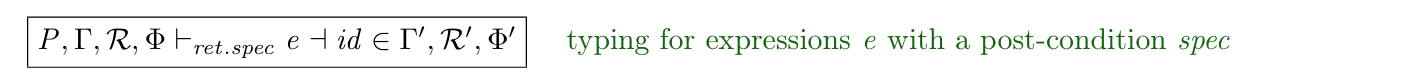
\includegraphics{figures/minicn-expr-judgement}
    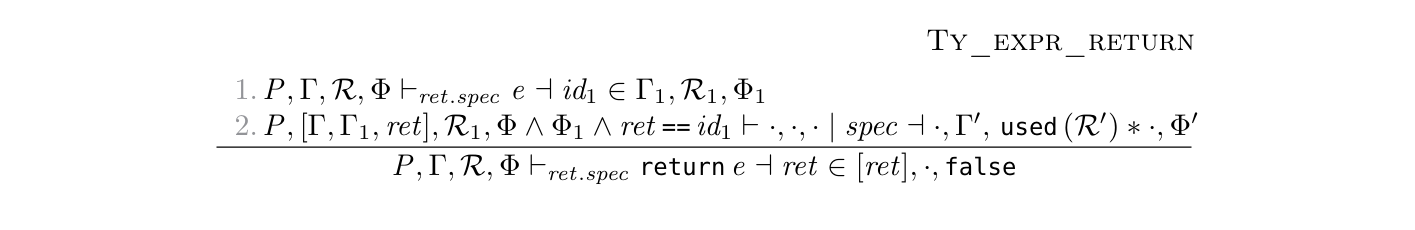
\includegraphics{figures/minicn-return}
    \caption{\kl{MiniCN} rule for typing a return expression.}\label{fig:minicn-return}
\end{figure*}

For the sake of simplicity, the synthesised value of each sub-expression is is
represented by a fresh variable and constrained in the output constraint
context. In the case of a return expression, the fresh variable remains
unconstrained and the output context has $\mathsf{false}$ added to it, to allow
any ancestor expression to continue typing correctly.

\begin{figure*}[tpb]
    \ContinuedFloat{}
    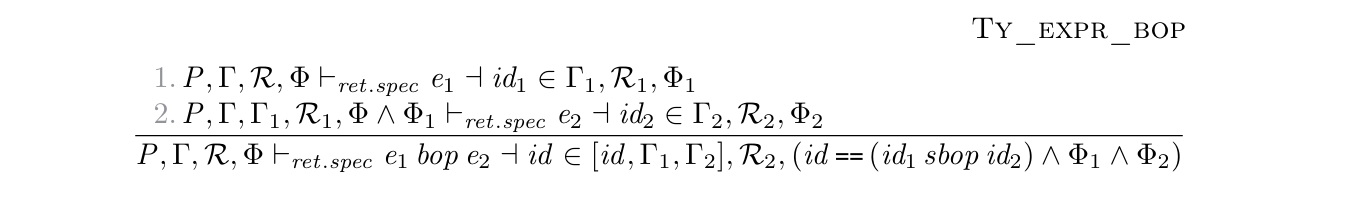
\includegraphics{figures/minicn-bop}
    \caption{\kl{MiniCN} rule for typing binary operations.}\label{fig:minicn-bop}
\end{figure*}

In the case of a binary operation expression (\cref{fig:minicn-bop}), this
shows how the let-normalisation absent in the grammar shows up in the
constraint context anyway.\sidenote{Remember that the implementation gets
around this by passing around explicit continuations
(\href{https://github.com/rems-project/cerberus/commit/350fefc675626dcc69c7adc9edea30ff9687b752}{commit
350fefc6}). Another way of implementing this would be to have the type
system's symbolic evaluation \emph{itself} specified as a non-determinism
monad (\href{https://github.com/rems-project/cerberus/issues/730}{issue
\#730}).}

\section{Lack of let-normalisation requires join-points}

Aside from complications arising from early returns, avoiding let-normalisation
also requires us to construct join-points for resource and constraint contexts
(\cref{fig:minicn-if}).

\begin{figure*}[tpb]
    \ContinuedFloat{}
    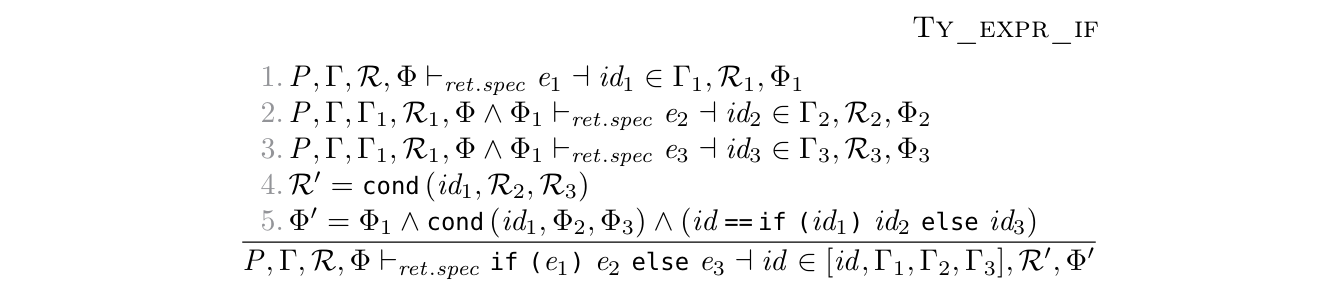
\includegraphics{figures/minicn-if}
    \caption{\kl{MiniCN} rule for typing an if-expressions.}\label{fig:minicn-if}
\end{figure*}

I chose to represent these join-points as an ordered-disjunction of
\emph{contexts}, both resource and constraint. This is not very satisfying,
because it complicates how to specify a lookup in the resource context. I
outlined a scheme where such ordered-disjunctions would be simplified if either
the condition or its negation could be proven, and otherwise require a
syntactic match on both branch.

\section{Discussion}

As I showed in the previous sections, the typing judgements for \kl{MiniCN}
becomes substantially more complicated in the absence of key features of
\kl{ResCore}. This would extend to the proof of soundness too, because\ldots
struggling to explain this.

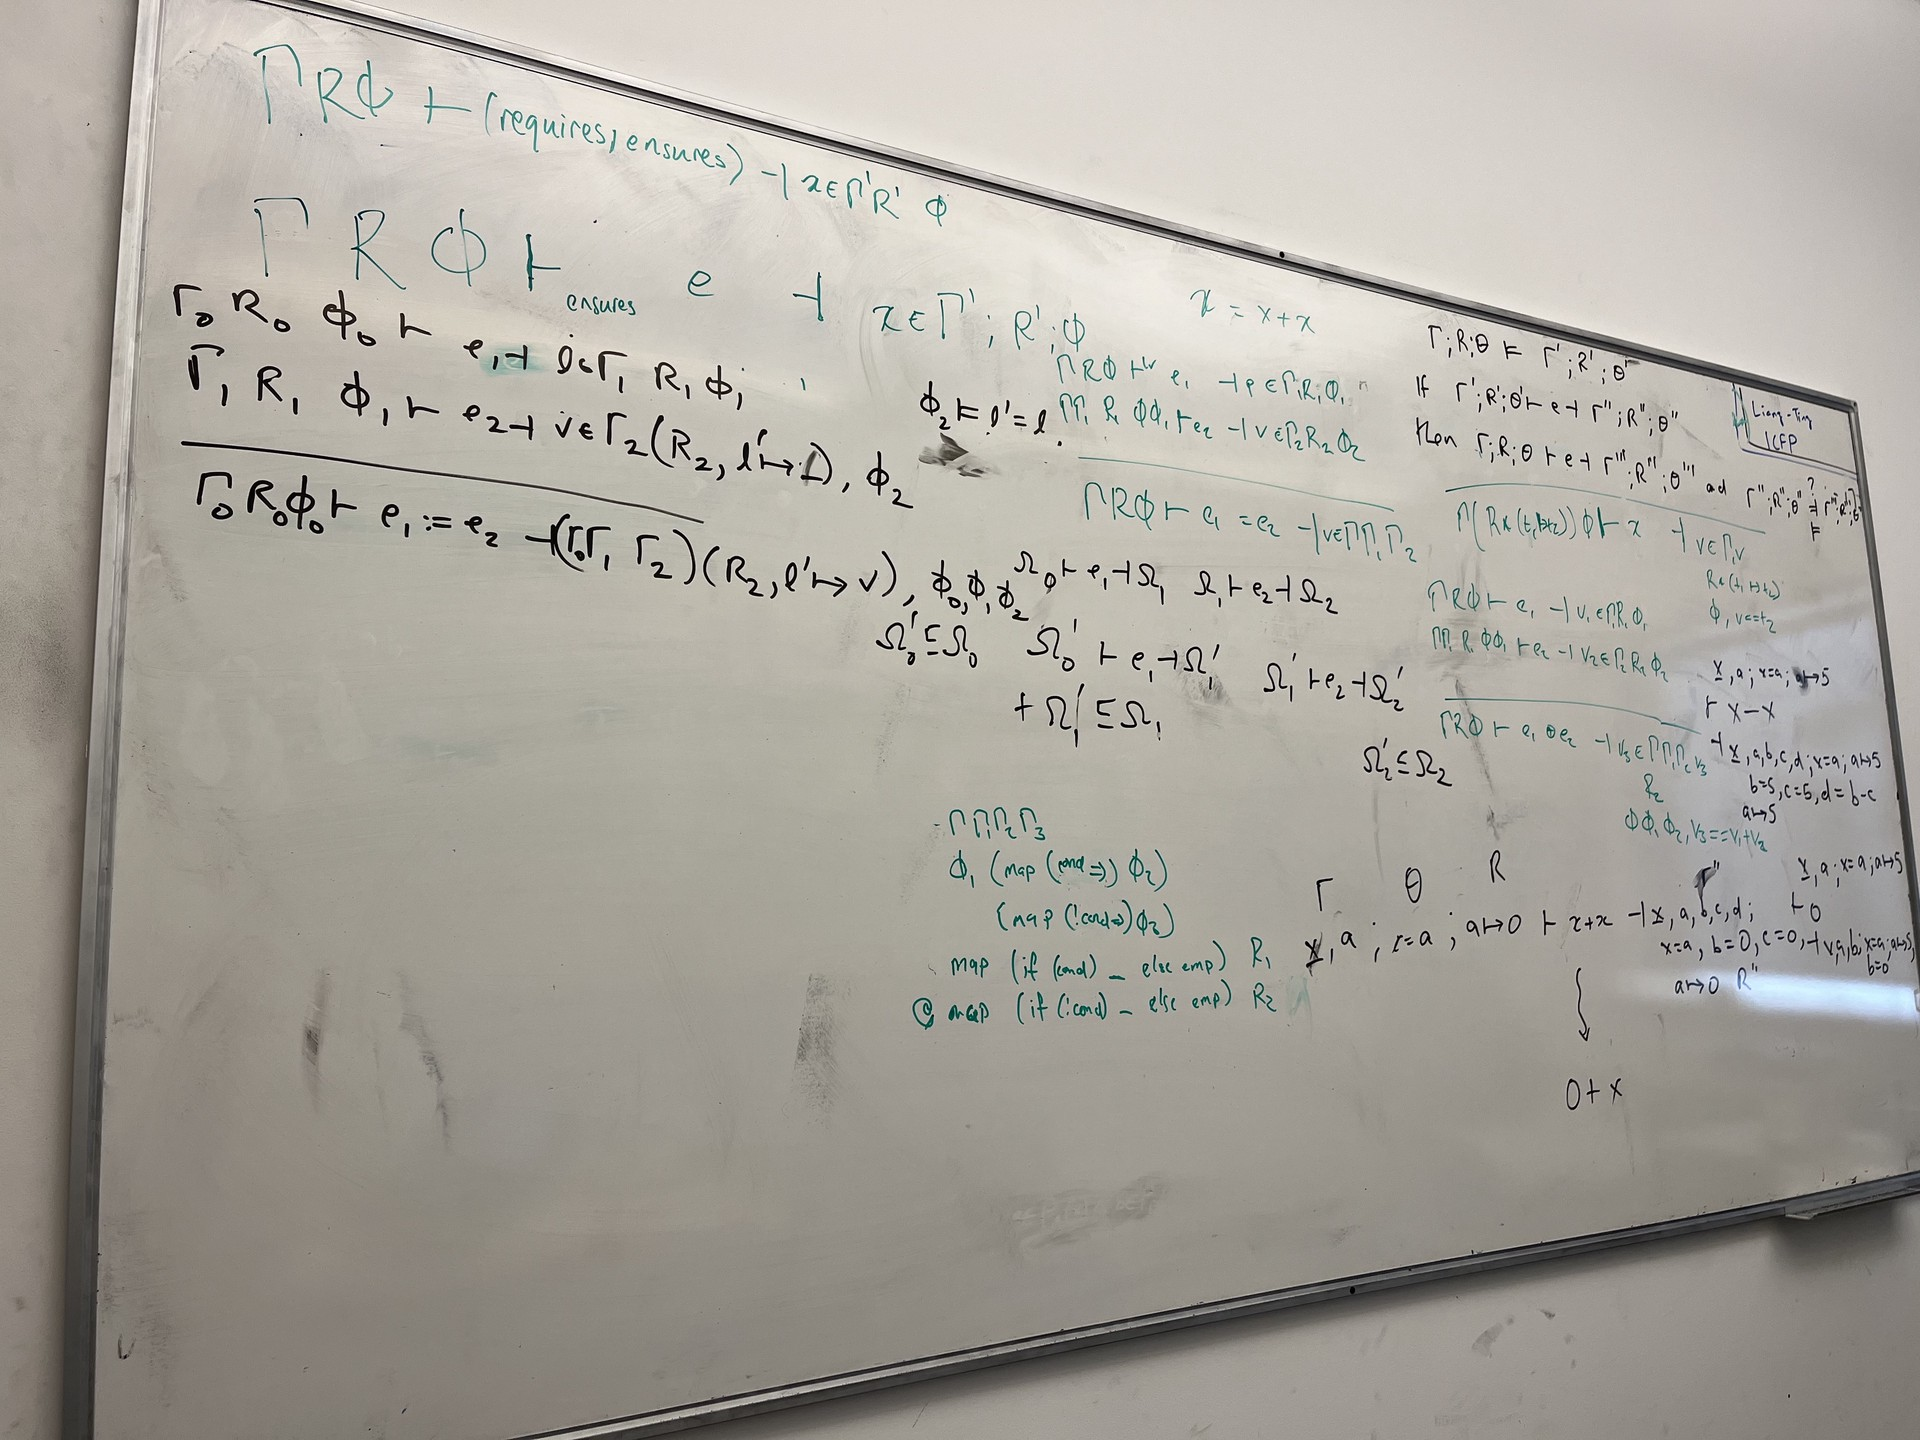
\includegraphics{../misc/minicn-soundness}

Or this

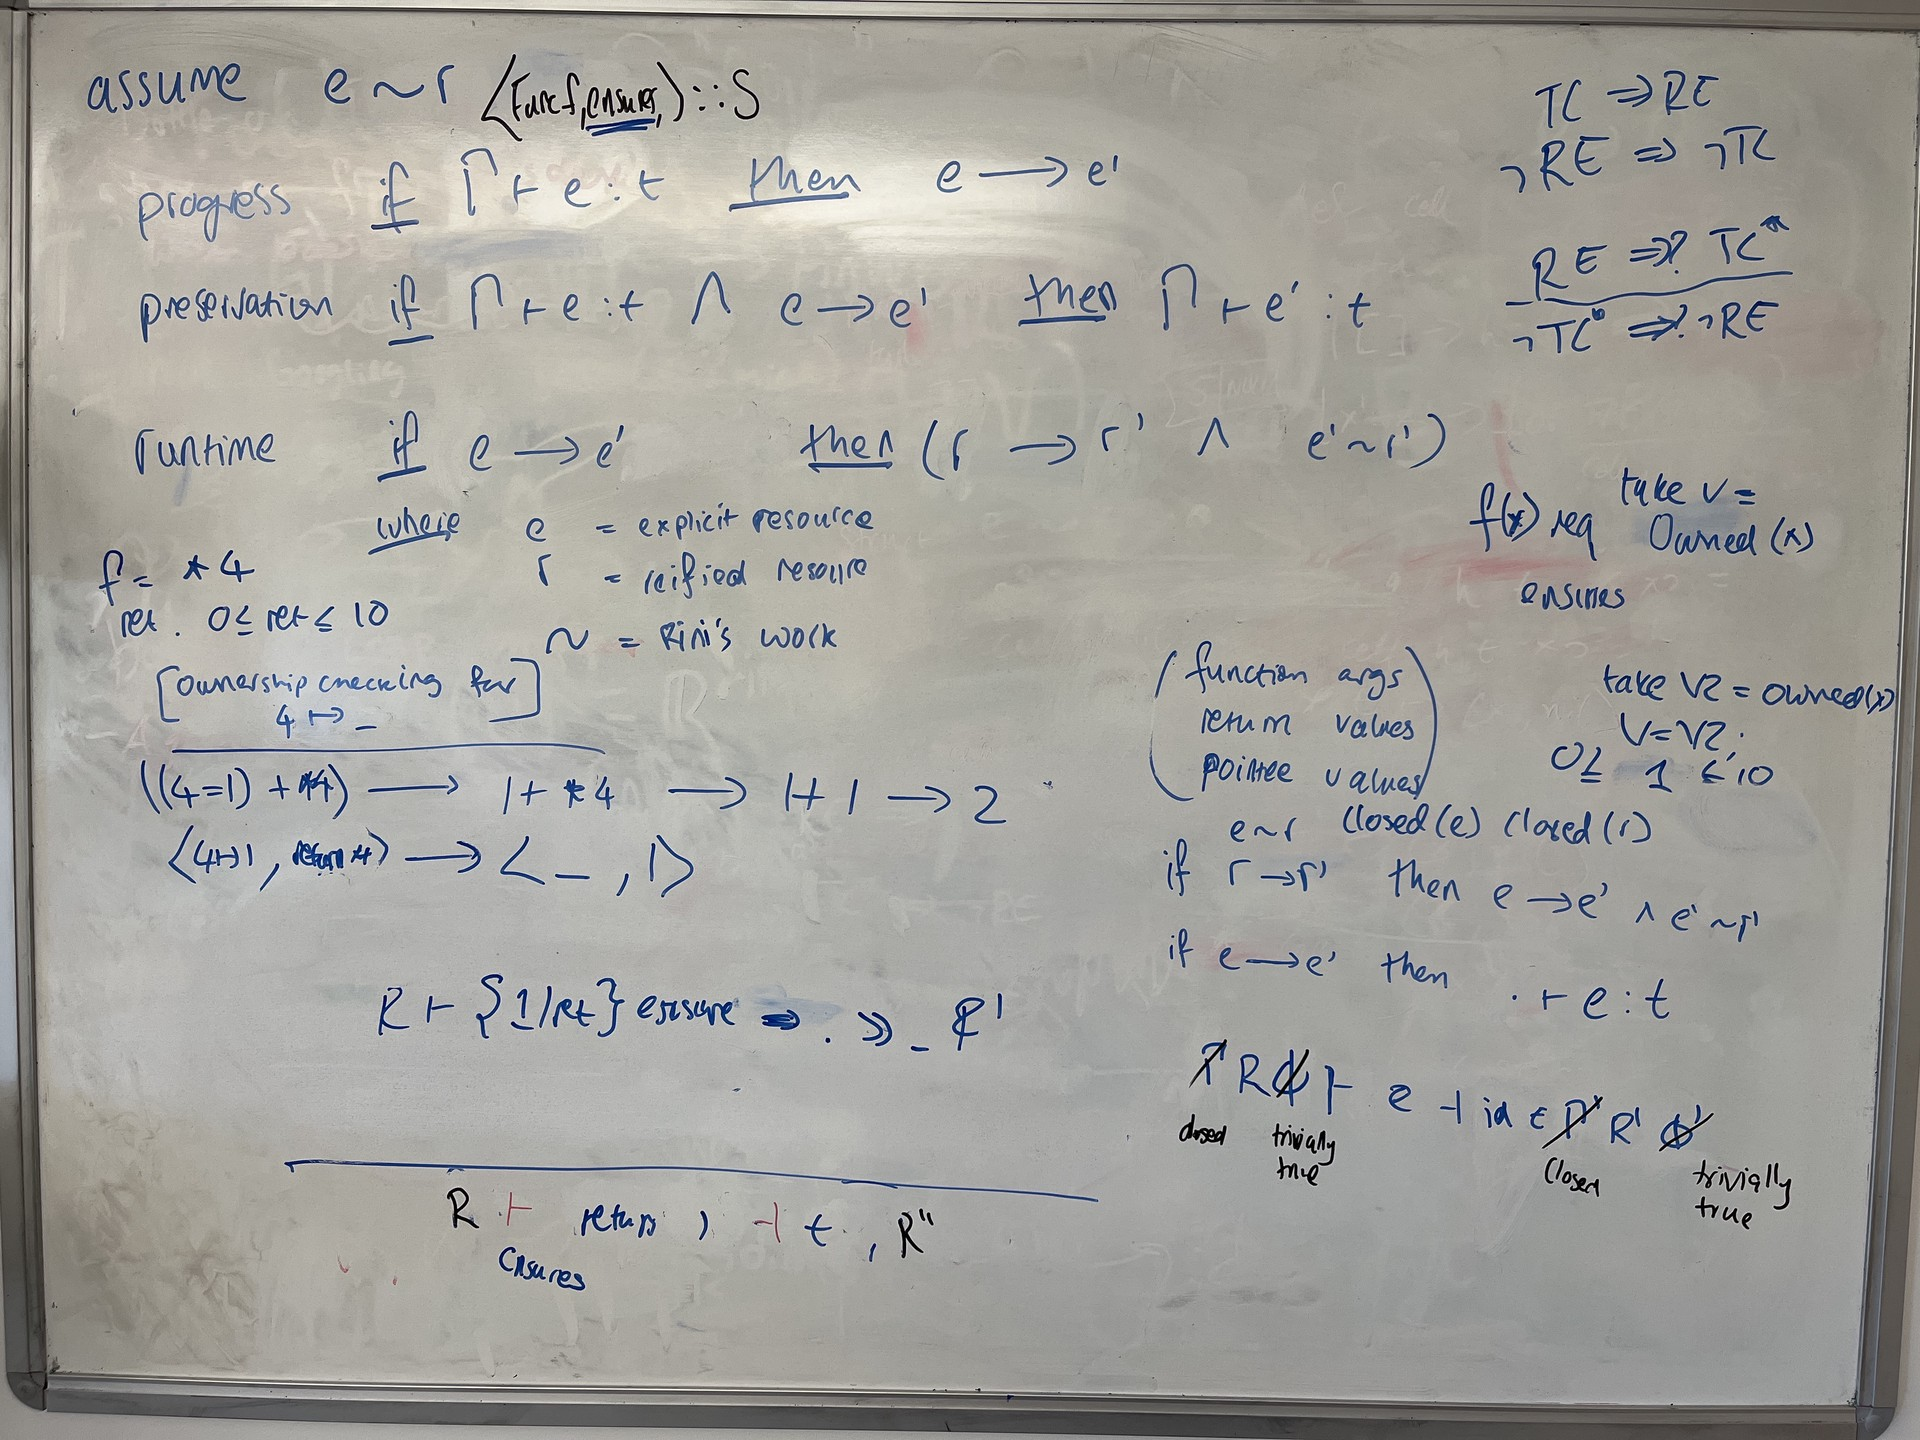
\includegraphics{../misc/runtime-correctness}

